\section{Control Charts with Memory}
\noindent\rule[\linienAbstand]{\linewidth}{\linienDickeDick}

\textbf{Classical Shewhart control charts}\\
Using a classic Shewhart control chart, the decision to interfere with the production process is based only on the results of the current sample.
The development of the manufacturing process in the past is not considered in the decision. On the other hand, control charts developed in recent years are also based on random samples taken in the past.
These charts are called control charts with memory.
Because these charts use more information about the process, they can detect a disturbance faster than the classical charts.\\

Control charts with memory are based on a linear combination of the mean values of some or all random samples taken up to the time with index $i$, i.e.
\begin{equation}
 y_i = \alpha_i + \sum_{j=1}^i \beta_j \bar{x}_j,
\end{equation}
where $\alpha_i$ and the weights $\beta_1, ..., \beta_i$ can be arbitrary real numbers where the sum of all $\beta s = 1$.\\
Depending on how the weights are chosen, we get another type of control chart.

\subsection{CUSUM - Cumulative Sum Control Chart}
\noindent\rule[\linienAbstand]{\linewidth}{\linienDicke}
\textbf{Idea}\\
The CUSUM chart plots the cumulative sums of deviations of measurement values from the target value.\\

\textbf{Recursive procedure}\\
Using two statistics $C^+$, resp. $C^-$ the CUSUM chart sums up deviations above, resp. below the target value
\begin{equation}
  \begin{split}
    C^+_i &= max\{0, \bar{x}_i - (\mu_0 + K) + C_{i-1}^+\},\\
    C^-_i &= max\{0, (\mu_0 - K) - \bar{x}_i + C_{i-1}^+\}.
  \end{split}
\end{equation}
$C^+$ and $C^-$ only sum up deviations from the target value, which are greater than the reference value $K$.
The starting values of the recursion are $C^+ = 0$ and $C^- = 0$.\\

If a shift of $\Delta$ is to be detected then set
\begin{equation}
  K = \frac{\Delta}{2}.
\end{equation}
The constant $K$ is called reference value.\\

If the process is under controll the expected values of the statistic are both 0.\\
If the process is not under control, then the statistic sums up the deviations. If the sum of de deviations ($C^+$ and $C^-$) exceed the decision interval $H$, then we should stop the process and look for the cause.\\

Rule of thumb for choosing the constants $K$ and $H$:
Let $\hat{\sigma}$ be an estimate for the process standard deviation.\\
\begin{itemize}
  \item reference value = $K \frac{\hat{\sigma}}{2}$
  \item decision interval $H = 5\hat{\sigma}$
\end{itemize}

\begin{figure}[H]
  \centering
  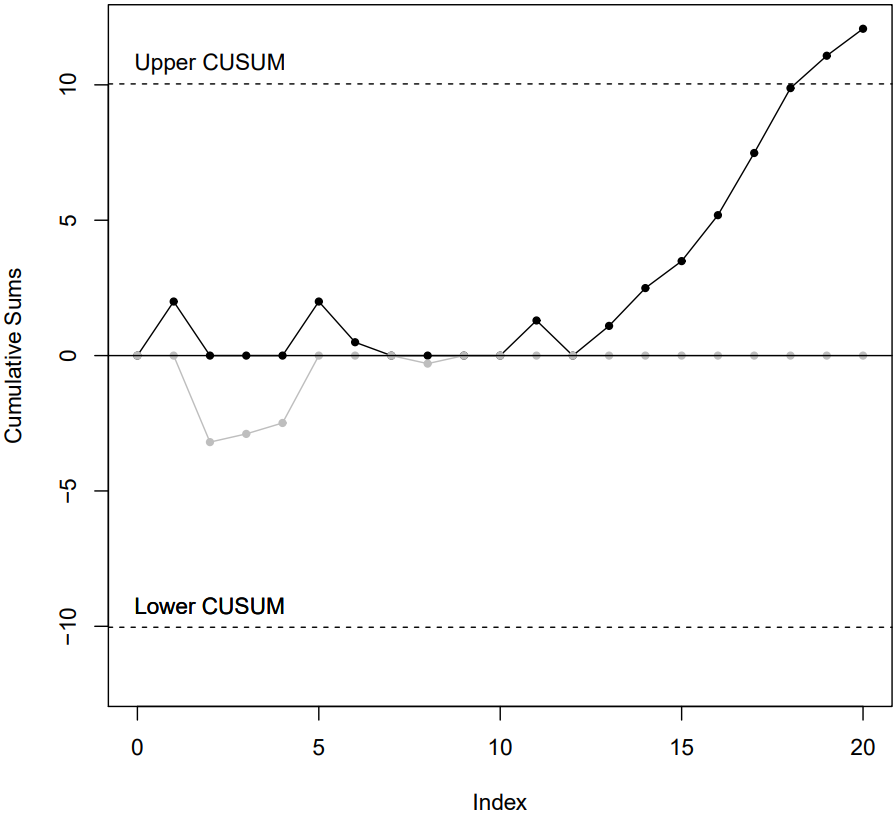
\includegraphics[width=0.8\linewidth]{Pics/4.1.png}
  \caption{CUSUM-Chart}
  \label{CUSUM}
\end{figure}


\subsection{EWMA - Exponentially Weighted Moving Average}
\noindent\rule[\linienAbstand]{\linewidth}{\linienDicke}
\textbf{Idea}\\
Monitor the mean and weight its influence on the statistic with the exponentially decaying factor $\beta_j$.\\

\textbf{Smoothing parameter $\lambda$}\\
Lambda lays between 0 and 1. The smoothing parameter $\lambda$ determines the influence of the previous sample mean $\bar{x}_j$ on the statistic. The smaller $\lambda$, the more values $\bar{x}_j$ are used for the decision. For $\lambda = 1$ only one sample is used and we get the well-known Shewhart $\bar{x}$ chart.\\

\textbf{Weights}\\
\begin{equation}
  \begin{split}
    \alpha_i =& (1-\lambda)^1 \mu_0\\
    \beta_j =& \lambda(1-\lambda)^{i-j} \text{with } j \in \{1,2,...,i\}.
  \end{split}
\end{equation}

\textbf{Statistics}\\
\begin{equation}
  y_i = (1-\lambda)^i \mu_0 + \lambda \sum_{j=1}^i(1-\lambda)^{i-j}\bar{x}_j
\end{equation}
Start: $y_0 = \mu_0$\\

\textbf{The same with recursion}\\
\begin{equation}
  y_i = (1-\lambda)y_{i-1} + \lambda\bar{x}_j
\end{equation}

\textbf{Assumptions}\\
If the process is under control, then $\bar{x}_i$ comes from a normal distribution with the expected value $\mu_0$ and the standard deviation $\frac{\sigma}{\sqrt{n}}$.\\
The standard deviation is either known or can be estimated from data. The statistic $y_i$ is then also normally distributed with $E(y_i) = \mu_0$ and
\begin{equation}
  Var(y_i) = \frac{\lambda}{2-\lambda}(1-(1-\lambda)^{2i})\frac{\sigma^2}{n}
\end{equation}

\textbf{Control limits}\\
These assumptions lead to the $3\sigma$ control limits:
\begin{equation}
  \begin{split}
    UCL_i =& \mu_0 + 3 \sqrt{\frac{\lambda}{2-\lambda}\left(1-(1-\lambda)^{2i}\right)}\frac{\sigma}{\sqrt{n}}\\
    LCL_i =& \mu_0 - 3 \sqrt{\frac{\lambda}{2-\lambda}\left(1-(1-\lambda)^{2i}\right)}\frac{\sigma}{\sqrt{n}}
  \end{split}
\end{equation}

The asymtotic control limits are:
\begin{equation}
  \begin{split}
    UCL_i =& \mu_0 + 3 \sqrt{\frac{\lambda}{2-\lambda}}\frac{\sigma}{\sqrt{n}}\\
    LCL_i =& \mu_0 - 3 \sqrt{\frac{\lambda}{2-\lambda}}\frac{\sigma}{\sqrt{n}}
  \end{split}
\end{equation}

\textbf{Estimate of process standard error}\\
\begin{equation}
  \hat{\sigma} = \frac{\bar{s}}{c_4}
\end{equation}

\begin{figure}[H]
  \centering
  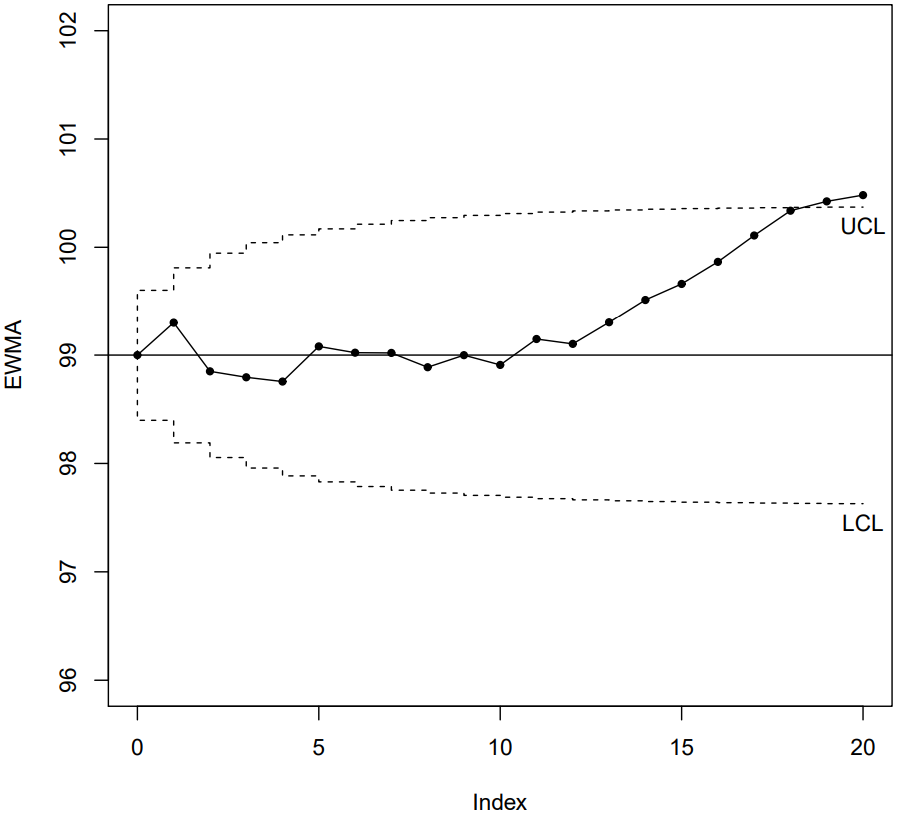
\includegraphics[width=0.8\linewidth]{Pics/4.2.png}
  \caption{EWMA-Chart}
  \label{EWMA}
\end{figure}
